\chapter{\ifproject%
\ifenglish Project Structure and Methodology\else โครงสร้างและขั้นตอนการทำงาน\fi
\else%
\ifenglish Project Structure\else โครงสร้างของโครงงาน\fi
\fi
}

\makeatletter

% \renewcommand\section{\@startsection {section}{1}{\z@}%
%                                    {13.5ex \@plus -1ex \@minus -.2ex}%
%                                    {2.3ex \@plus.2ex}%
%                                    {\normalfont\large\bfseries}}

\makeatother
%\vspace{2ex}
% \titleformat{\section}{\normalfont\bfseries}{\thesection}{1em}{}
% \titlespacing*{\section}{0pt}{10ex}{0pt}

\section{การใช้งานพื้นฐาน}
ในส่วนของโมไบล์แอปพลิเคชัน เป็นเครื่องมือที่จะจำเป็นต้องใช้งานกล้องและบันทึกพิกัดตำแหน่งทาง GPS อยู่ตลอดเวลาเพื่อทำการส่งรูปภาพ 
พร้อมกับพิกัดตำแหน่ง แล้วนำไประมวลผลในเซอร์วิสที่ได้ออกแบบเอาไว้ โดยที่เซอร์วิสดังกล่าวจะทำการประมวลผลรูปภาพเพื่อหาป้ายโฆษณาที่สามารถจัดเก็บภาษีได้ 
และหลังจากนั้นก็จะจัดเก็บลงฐานข้อมูลต่อไป 

ในส่วนของเว็บแอปพลิเคชัน จะเป็นส่วนของการแสดงผลข้อมูลที่ได้บันทึกมาได้ส่วนของโมไบล์แอปพลิเคชัน โดยจะแสดงในรูปแบบของหมุดในแผนที่ 
คล้าย ๆ กับการปักหมุดของ Google map โดยที่ในแต่ละหมุดสามารถกดเพื่อดูรายละเอียดต่าง ๆ ได้ เช่น พิกัดของหมุดนั้น 
และลักษณะรูปป้ายในตำแหน่งนั้นๆที่ได้บันทีกมาจากโมไบล์แอปฯ 

\section{การออกแบบระบบพื้นฐานของโครงงาน}
\subsection{Database Design}
ประกอบด้วย 4 ตารางดังรูปที่ 3.1 ได้แก่
\begin{enumerate}
  \item User table: เนื่องจากระบบต้องมีการ Authentication เพื่อเข้าใช้งานไม่ว่าจะเป็นทั้งส่วนของ โมไบล์แอปฯ หรือเว็บแอปฯ 
  ดังนั้นตารางนี้จึงจะใช้เก็บข้อมูลพืื้นฐานต่าง ๆ ที่จำเป็นต่อการยืนยันตัวตนทั้งหมด 
  \item Role table: ใช้ในการเก็บบทบาททั้งหมดที่มีของระบบ เช่น ผู้ดูแลระบบ ผู้สำรวจ และอื่น ๆ 
  \item Asset table: ใช้ในการเก็บข้อมูลที่ได้รับมาจาก โมไบล์แอปฯ ไม่ว่าจะเป็นตำแหน่งของรูป ชื่อของรูป และประเภทของ asset ที่ตรวจจับได้ 
  \item Asset type table: ใช้ในการเก็บประเภทของ asset ต่างๆที่ระบบสามารถตรวจจับได้ 
  \item Config table: ใช้เก็บการตั้งค่าพื้นฐานต่างๆเช่น ขอบเขตของแผนที่ 
\end{enumerate}

\begin{figure}[ht]
  \begin{center}
  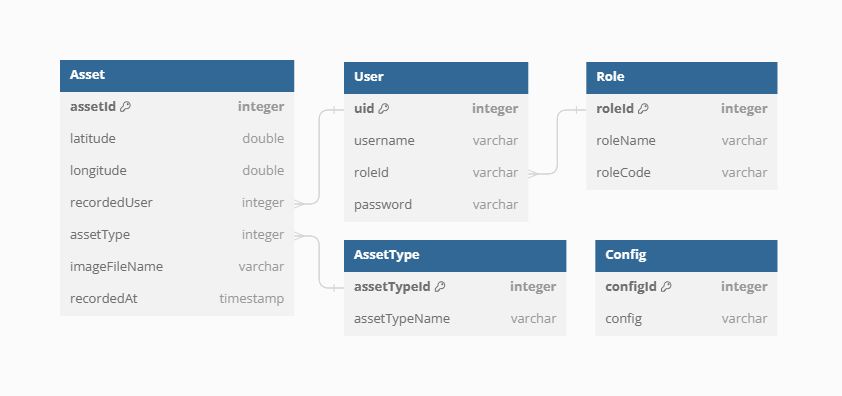
\includegraphics[scale=0.8]{resources/ScreetnerDB.png}
  \end{center}
  \caption[Database Design]{Overall Database Design}
  \label{fig:database}
\end{figure}

% TODO: DELETE IF NECESSARY
\newpage
\subsection{System Design}
จากรูป จะอธิบายถึงโครงสร้างระบบของโครงงานงานนี้ในรูปแบบ Flow diagram เพื่อให้เข้าใจถึงโครงสร้างการทำงานพอสังเขป 
โดยที่ซอฟต์แวร์จะประกอบด้วย 3 ส่วนหลัก ๆ ได้ Mobile application ซึ่งจะทำงานตามรูปที่ 3.2 Web application ซึ่งจะทำงานตามรูปที่ 3.3 
และ Processing server โดยที่ลักษณะการทำงานร่วมกันระหว่างทั้งสามส่วนประกอบ แสดงตามรูปที่ 3.1 

\begin{figure}[ht]
  \begin{center}
  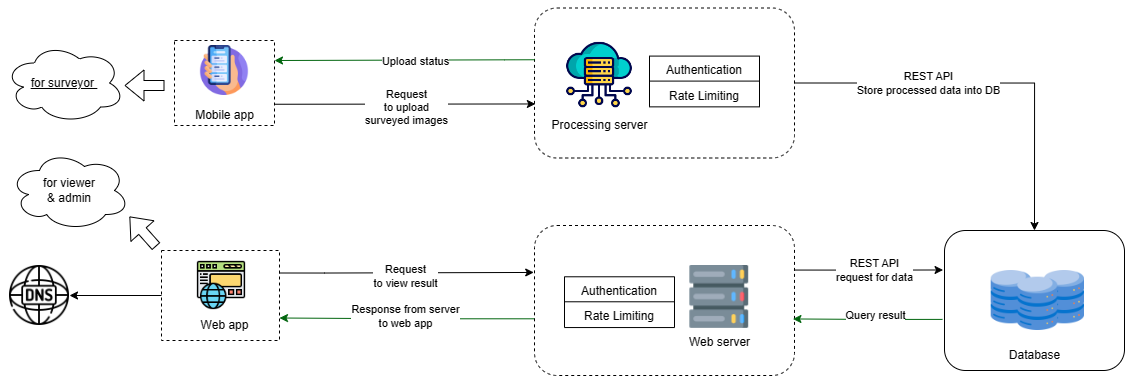
\includegraphics[scale=0.45]{resources/SystemDesign.png}
  \end{center}
  \caption[System Design]{Overall System Design}
  \label{fig:system design}
\end{figure}

% TODO: DELETE IF NECESSARY
\newpage
\subsection{Web Application Flow Diagram}
จากรูปที่ 3.3 จะอธิบายถึงลำดับการทำงานของเว็บแอปพลิเคชั่นในรูปแบบของ flow diagram เพื่อให้เข้าใจในลำดับการทำงานอย่างพอสังเขป 
พอหลังจากที่ได้เข้าระบบสู้หน้า dashboard จะมีตัวเลือกที่สามารถทำทำได้อยู่ 3 อย่างคือ filter เป็นการคัดกรองข้อมูลให้เหลือเพียงข้อมูลในช่วงเวลาที่เราต้องการ 
asset เป็นการกดที่รูปภาพเพื่อที่จะดูข้อมูลที่เกี่ยวกับ asset ดังกล่าว และ icon เป็นส่วนที่จะแสดงตัวเลือกเพิ่มเติมอีก 4 ทางเพื่อให้เราสามารถเลือกเข้าไปยังหน้าอื่นต่อไปได้

\begin{figure}[ht]
  \begin{center}
  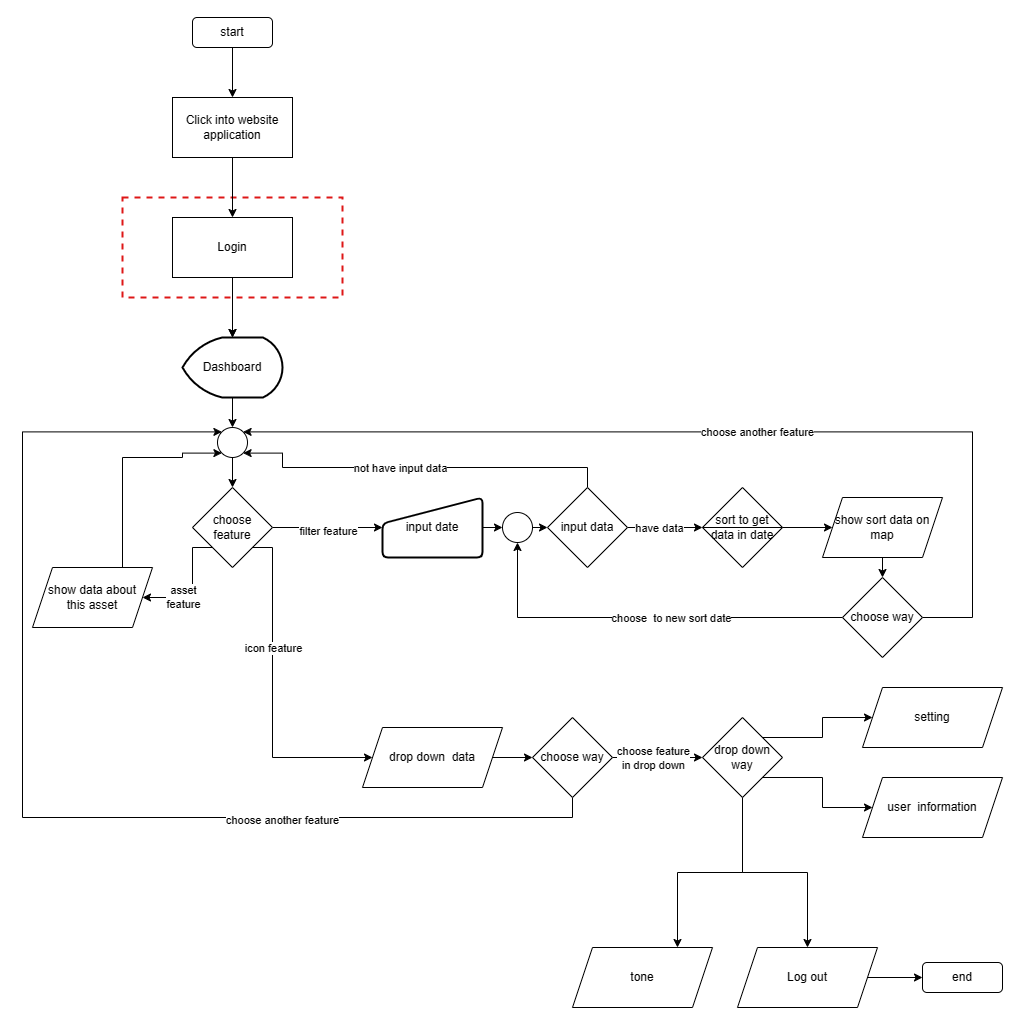
\includegraphics[scale=0.65]{resources/WebsiteFlow.png}
  \end{center}
  \caption[Web Application Flow Diagram]{Web Application Flow Diagram}
  \label{fig:web-app flow design}
\end{figure}

% TODO: DELETE IF NECESSARY
\newpage
\subsection{Mobile Application Flow Diagram}
รูปที่ 3.4 จะอธิบายถึงลำดับการทำงานขอโมไบล์แอปพลิเคชั่นในรูปแบบของ flow diagram เพื่อให้เข้าใจในลำดับการทำงานอย่างพอสังเขป โดยพอผู้ใช้จะเริ่มเข้าใช้งานแอปพลิเคชั่น 
ผู้ใช้จะต้องผ่านการเข้าสู่ระบบ ซึ่งมีขั้นตอนการทำงานดังรูปที่ 3.5 เพื่อเป็นการยืนยันตัวตน หลังจากที่ได้เข้าสู่แอปพลิเคชั่นเรียบร้อยแล้ว 
ผู้ใช้งานจะสามารถเริ่มสตรีมวิดีโอเพื่อทำการส่งรูปภาพในช่วงเวลาหนึ่งพร้อมแนบตำแหน่งพิกัดในช่วงเวลาดังกล่าวไปยังเซอร์วิสที่ได้จัดเตรียมเอาไว้อยู่ตลอดเวลาที่ทำการสตรีม 
เพื่อให้ทางเซอร์วิสทำการคืนค่าออกมาว่าในตำแหน่งนี้จะมี asset อยู่เท่าไหร่ โดยจะมีขั้นตอนการทำงานดังรูปที่ 3.6 
ซึ่งสิ่งที่คืนค่ามาทุกครั้งนั้นจะเอามาจัดเก็บเอาไว้บนมือถือชั่วคราวและยังไม่ได้ทำการบันทึกข้อมูลลงไปในฐานข้อมูลเพื่อให้ผู้ใช้งานสามารถดูข้อมูลได้ตลอดเวลาว่าปัจจุบันมี 
asset อยู่เท่าไหร่จนจบการทำงาน และในตอนท้ายของการทำงานผู้ใช้สามารถที่จะเลือกได้ว่าจะทำการสตรีมต่ออีกครั้งหรือไม่ หากไม่ทำการสตรีมต่อ 
ผู้ใช้งานต้องเลือกว่าจะทำการส่งข้อมูลทั้งหมดที่ได้มานั้นไปยังฐานข้อมูลหรือไม่
\begin{figure}[ht]
  \begin{center}
  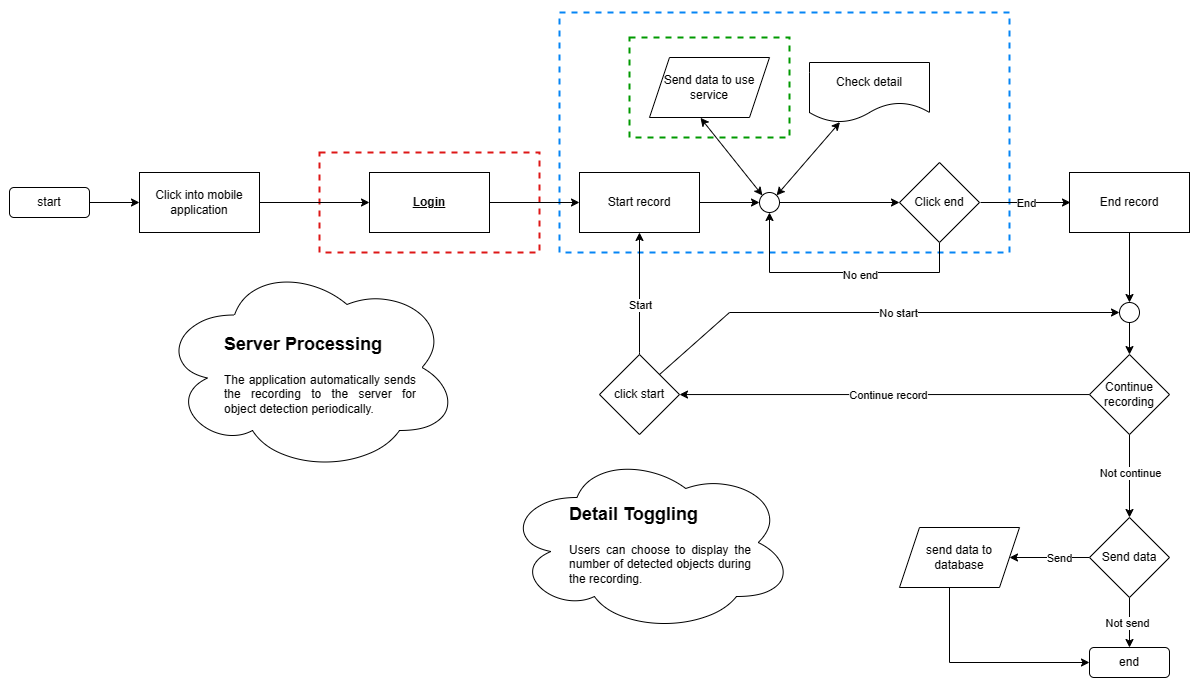
\includegraphics[scale=0.5]{resources/MobileAppFlow.png}
  \end{center}
  \caption[Mobile Application Flow Diagram]{Mobile Application Flow Diagram}
  \label{fig:mopile-app flow design}
\end{figure}

\begin{figure}[ht]
  \begin{center}
  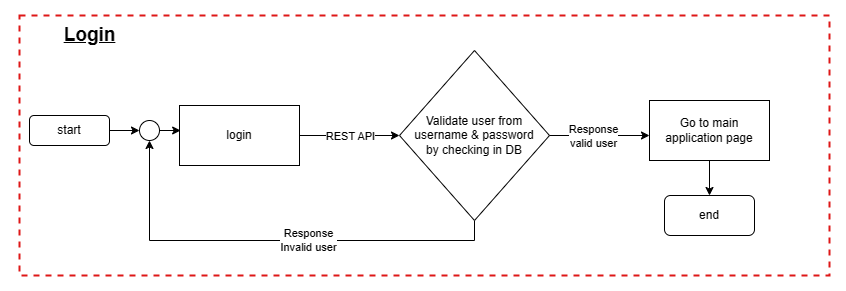
\includegraphics[scale=0.6]{resources/LoginFlow.png}
  \end{center}
  \caption[Login Flow Diagram]{Login Flow Diagram}
  \label{fig:login flow design}
\end{figure}

\begin{figure}[ht]
  \begin{center}
  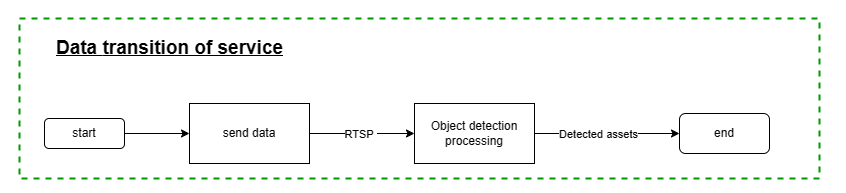
\includegraphics[scale=0.6]{resources/TransitionFlow.png}
  \end{center}
  \caption[Transition Flow Diagram]{Transition Flow Diagram}
  \label{fig:transition flow design}
\end{figure}
